\documentclass[prd,preprintnumbers,twocolumn,eqsecnum,floatfix,a4paper,nofootinbib,superscriptaddress]{revtex4}
\usepackage{color}
\usepackage{calc}
\usepackage{amsmath,amssymb,graphicx}
\usepackage{amssymb,amsmath}
\usepackage{bm}
\usepackage{microtype}
\usepackage{booktabs}
\usepackage{times}
\usepackage[varg]{txfonts}
\usepackage[colorlinks, pdfborder={0 0 0}]{hyperref}
\usepackage[utf8]{inputenc}
\definecolor{LinkColor}{rgb}{0.75, 0, 0}
\definecolor{CiteColor}{rgb}{0, 0.5, 0.5}
\definecolor{UrlColor}{rgb}{0, 0, 0.75}
\hypersetup{linkcolor=LinkColor}
\hypersetup{citecolor=CiteColor}
\hypersetup{urlcolor=UrlColor}
\maxdeadcycles=1000
\allowdisplaybreaks
\textwidth 7 in
\hoffset -0.1in
\textheight 10in
\DeclareFontFamily{OT1}{pzc}{}
\DeclareFontShape{OT1}{pzc}{m}{it}{<-> s * [1.10] pzcmi7t}{}
\DeclareMathAlphabet{\mathpzc}{OT1}{pzc}{m}{it}
\newcommand{\comment}[1]{\textcolor{blue}{\textit{#1}}}
\newcommand{\ajith}[1]{\textcolor{red}{\textit{Ajith:#1}}}
\newcommand{\checkthis}{\textcolor{magenta}{(CHECKTHIS)}}
\newcommand{\vijay}[1]{\textcolor{cyan}{Vijay: #1}}
\newcommand{\io}{\iota}
\newcommand{\p}{\phi}
\newcommand{\vp}{\varphi}

\newcommand{\h}{\mathpzc{h}}
\newcommand{\Hhat}{\hat{\mathpzc{H}}}
\newcommand{\B}{\mathpzc{B}}
\newcommand{\hlm}{\mathpzc{h}_{\ell m}}
\newcommand{\xilm}{\xi_{\ell m}}
\newcommand{\Ylm}{{Y}^{-2}_{\ell m}}
\newcommand{\Y}{{Y}^{-2}}
\newcommand{\hc}{h_\times}
\newcommand{\hp}{h_+}
\newcommand{\Fc}{F_\times}
\newcommand{\Fp}{F_+}
\newcommand{\Mf}{M_f}
\newcommand{\cA}{\mathpzc{A}}
\newcommand{\lm}{_{\ell m}}
\newcommand{\deff}{d_\mathrm{eff}}
\newcommand{\rmi}{\mathrm{i}}
\newcommand{\blambda}{\bm{\lambda}}
\newcommand{\btheta}{\bm{\theta}}
\newcommand{\Mo}{M_{\odot}}
\newcommand{\FFe}{\mathrm{FF}_\mathrm{eff}}
\newcommand{\FF}{\mathrm{FF}}
\newcommand{\e}{\mathrm{e}}
\newcommand{\rhoopt}{\rho_\mathrm{opt}}
\newcommand{\rhosubopt}{\rho_\mathrm{subopt}}
\newcommand{\fqnm}{f}
\newcommand{\sigmaqnm}{\sigma}

\newcommand*{\skymapscale}{0.5}
\newcommand*{\paramestscale}{0.455}

\begin{document}

\newcommand{\be}{\begin{equation}}
\newcommand{\ee}{\end{equation}}
\newcommand{\ber}{\begin{eqnarray}}
\newcommand{\eer}{\end{eqnarray}}
\def\bea{\begin{eqnarray}}
\def\eea{\end{eqnarray}}
\newcommand{\etal}{\emph{et al}}

\title{Accurate inspiral-merger-ringdown gravitational waveforms \\ for non-spinning black-hole binaries including the effect of subdominant modes}
% \author{Ajit Kumar Mehta}
% \affiliation{International Centre for Theoretical Sciences, Tata Institute of Fundamental Research, Bangalore 560012, India}
% \author{Chandra Kant Mishra}
% \affiliation{International Centre for Theoretical Sciences, Tata Institute of Fundamental Research, Bangalore 560012, India}
% \affiliation{Indian Institute of Technology, Madras, Chennai 600036, India}
% \author{Vijay Varma}
% \affiliation{Theoretical Astrophysics, 350-17, California Institute of Technology, Pasadena, CA 91125, USA}
% \affiliation{International Centre for Theoretical Sciences, Tata Institute of Fundamental Research, Bangalore 560012, India}
% \author{Parameswaran~Ajith}
% \affiliation{International Centre for Theoretical Sciences, Tata Institute of Fundamental Research, Bangalore 560012, India}
% \affiliation{Canadian Institute for Advanced Research, CIFAR Azrieli Global Scholar, MaRS Centre, West Tower, 661 University Ave., Suite 505, Toronto, ON M5G 1M1, Canada}

\begin{abstract}
\end{abstract}
\preprint{LIGO-P1700160-v3}
\maketitle
%%%%%%%%%%%%%%%%%%%%%%%%%%%%%%%%%%%%%%%%%%%%%%%%%%%%%%%%%%%%%%%%%%%%%%%%%%%%%%%%%%%%%%%%%%%%%%%%%%%%%%%%%%%%%%%%%%%%%%%%%%%%%%%%%%%%%%%%%%%%%%%`
\section{Introduction}
%%%%%%%%%%%%%%%%%%%%%%%%%%%%%%%%%%%%%%%%%%%%%%%%%%%%%%%%%%%%%%%%%%%%%%%%%%%%%%%%%%%%%%%%%%%%%%%%%%%%%%%%%%%%%%%%%%%%%%%%%%%%%%%%%%%%%%%%%%%%%%%`
\section{Consistency between spherical harmonic modes}
\subsection{Consistency between parameters estimated from different modes}
%%%%%%%%%%%%%%%%%%%%%%%%%%%%%%%%%%%%%%%%%%%%%%%%%%%%%%%%%%%%%%%%%%%%%%%%%%%%%%%%%%%%%%%%%%%%%%%%%%%%%%%%%%%%%%%%%%%%%%%%%%%%%%%%%%%%%%%%%%%%%%%`
\subsection{Consistency between the amplitude and phase from different modes}
We split the contributions from the dominant $(\ell = 2, m = \pm 2)$ mode of gravitational radiation, and the higher order modes 
\begin{eqnarray}
\h(t; \n, \blambda, \Delta \blambda) & = & \sum_{m = \pm2} Y^{-2}_{2m} (\n) {\h}_{2m}(t, \blambda)  \nonumber \\ 
& + & \sum _{\text{H.O.M}} (1+\Tilde{c_1})\Ylm (\n) \hlm(t, \blambda)
\label{eq:test_amp}
\end{eqnarray}
where  H.O.M represents the higher order modes, and $\blambda$ the intrinsic parameters (say, chirp mass $M_c$ and mass ratio $q$). We introduce a deviation parameter $\Tilde{c_1}$ in H.O.M amplitudes, where $\Tilde{c_1}$ is complex in nature. We estimate $\Tilde{c_1}$ in addition to the standard set of intrinsic and extrinsic parameters in general relativity (GR). $\Tilde{c_1}$ would be zero for GR.

\newpage 
\noindent Corner plot  - Fig \ref{fig:c1_corner};\\
triangle plot - Fig \ref{fig:c1_triangle};\\
90\% credible intervals of $\Tilde{c_1}$  - Fig \ref{fig:c1_bound_a}, Fig \ref{fig:c1_bound_b} \& Fig \ref{fig:c1_bound_c}
\newpage

\begin{figure}[tbh]
\begin{center}
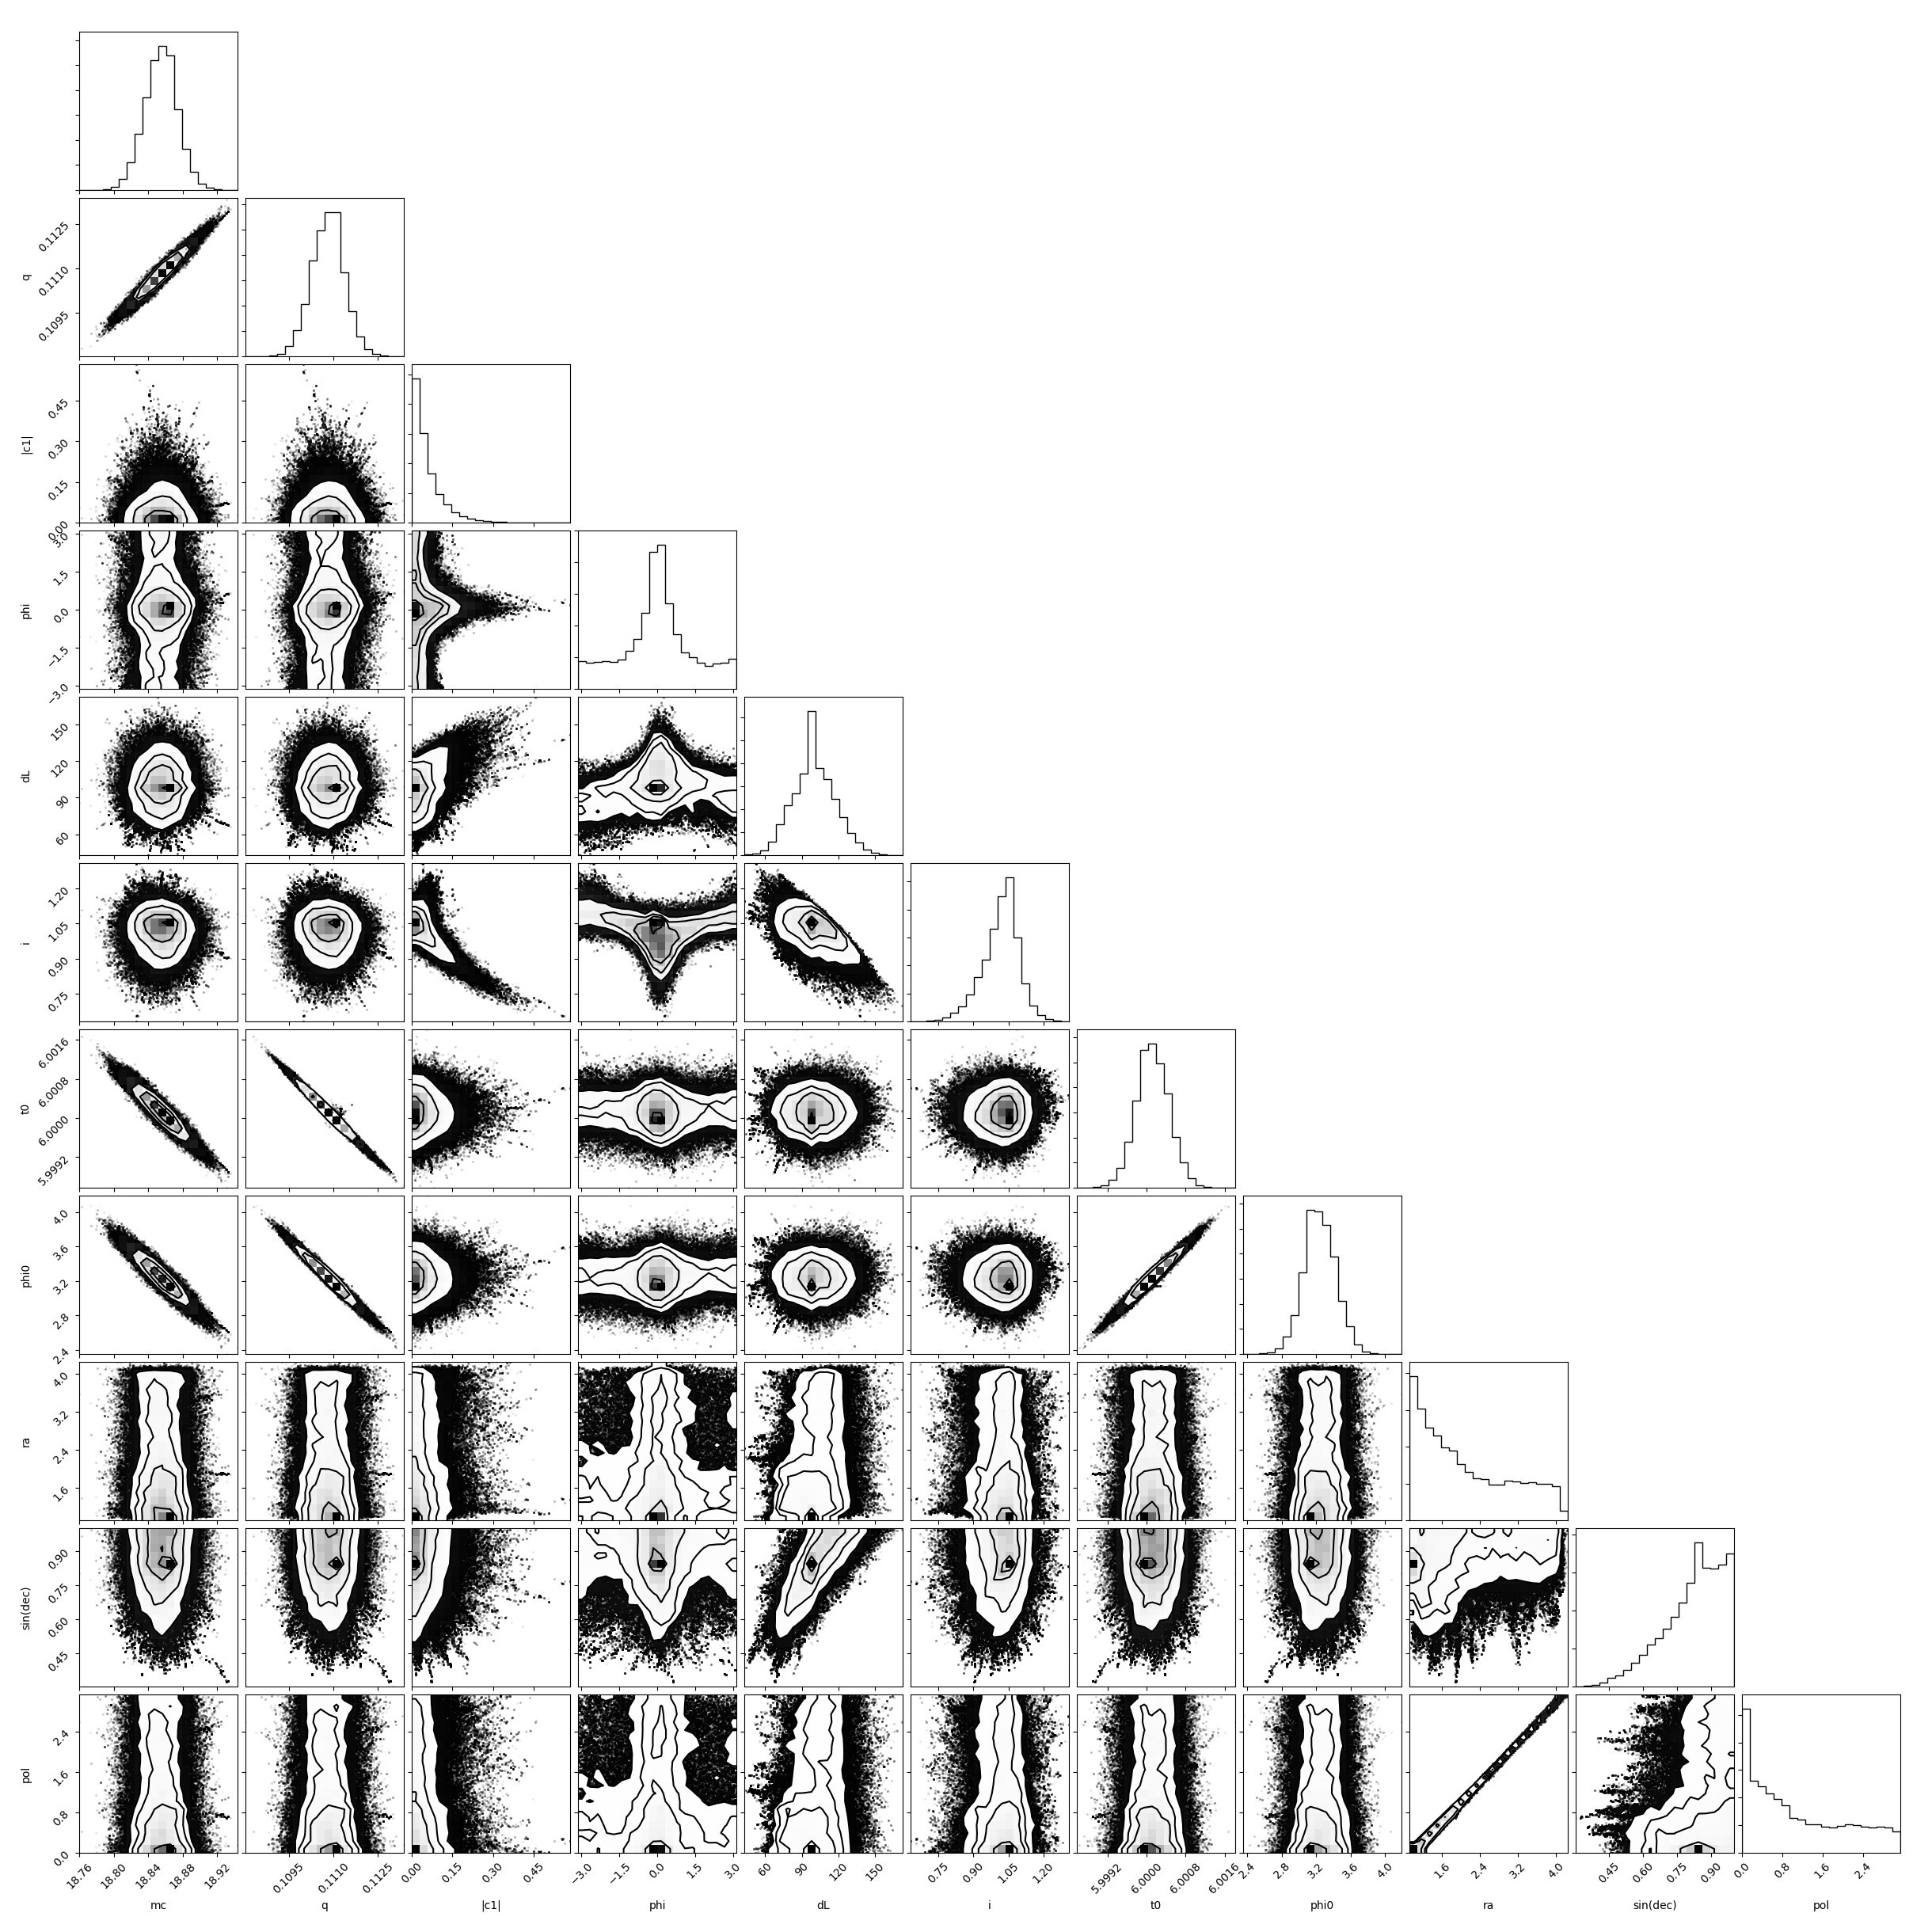
\includegraphics[scale=0.25]{figs/c1_80_9_100_corner_plot_wo_burnin.png} 
\end{center} 
\caption{Corner plot for tests of GR with complex deviation parameter $c_1$ in the higher order modes. M=80, q=9 and SNR=100.}
\label{fig:c1_corner}
\end{figure}

\newpage
.
\newpage 


\begin{figure}[tbh]
    \begin{center}
    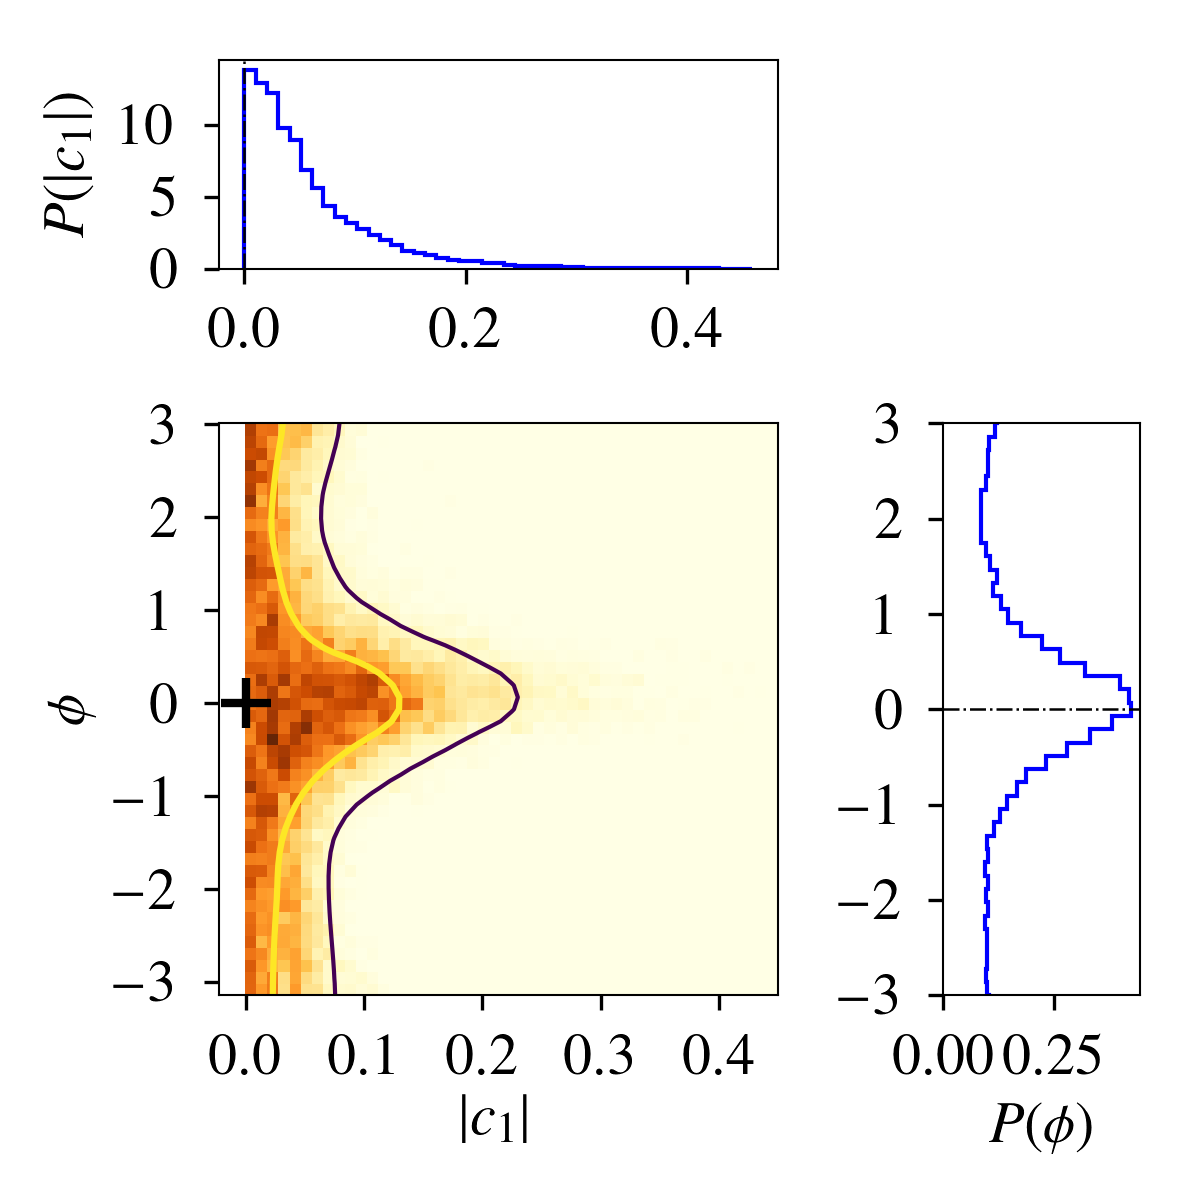
\includegraphics[scale=0.8]{figs/triangle_plot_M_80_q_9_snr_100_complex_c1.png}
    %
\includegraphics[scale=0.75]{figs/triangle_plot_M_80_q_9_snr_100_complex_c1.pdf}
    \end{center} 
    \caption{The middle plot shows the 50\% and 90\% credible regions in joint posteriors of two parameters: amplitude $|c_1|$ and phase $\phi$ of the complex deviation parameter $c_1$ estimated from different simulated GR signal corresponding to a binary with total mass $M=80$ $M_{\odot}$ , mass ratio $q=9$ and SNR 100.}
    \label{fig:c1_triangle}
\end{figure}

\begin{figure}[h]
    \begin{center}
    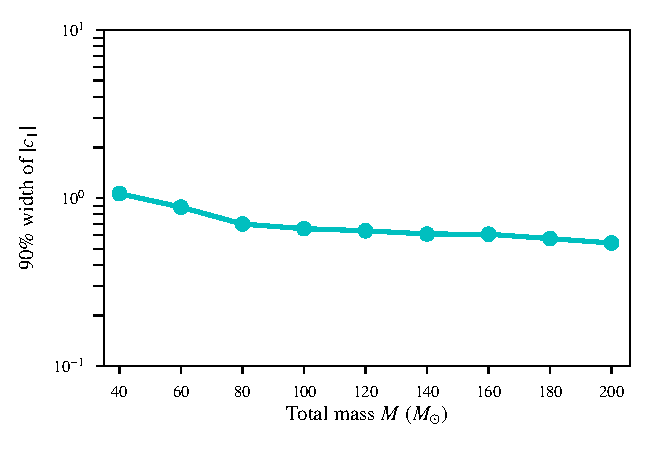
\includegraphics[scale=0.75]{figs/confidence_interval_c1_varying_M_q_9_snr_25.pdf} 
    \end{center} 
    \caption{The plots shows the width of the 90\% credible region of $|c_1|$ as a function of total mass $M$. All binaries correspond to a mass ratio $q = 1/9$ and SNR 25.}
    \label{fig:c1_bound_a}
\end{figure}

\begin{figure}[h]
    \begin{center}
    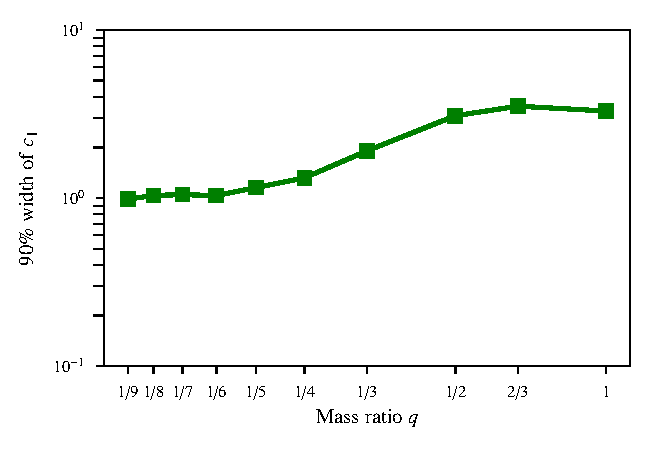
\includegraphics[scale=0.75]{figs/confidence_interval_c1_varying_q_M_40_snr_25.pdf} 
    \end{center} 
    \caption{The plots shows the width of the 90\% credible region of $|c_1|$ as a function of mass ratio $q$. All binaries correspond to a mass ratio $M = 40$ $M_{\odot}$ and SNR 25.}
    \label{fig:c1_bound_b}
\end{figure}

\newpage
\begin{figure}[h]
    \begin{center}
    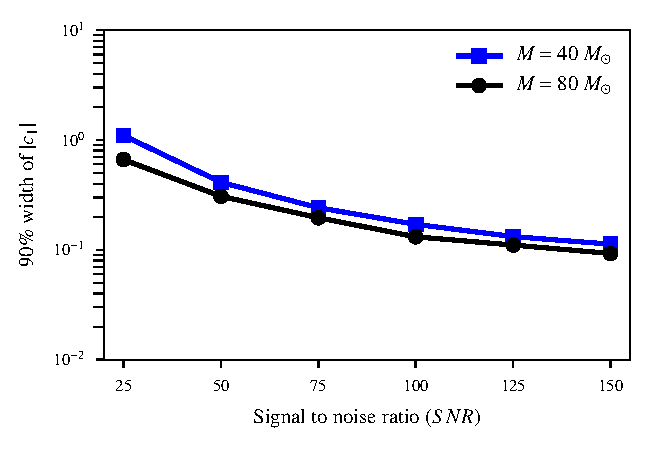
\includegraphics[scale=0.75]{figs/confidence_interval_c1_varying_snr.pdf} 
    \end{center} 
    \caption{The plots shows the width of the 90\% credible region of of $|c_1|$ as a function of signal to noise ratio. All binaries correspond to a mass ratio $q = 1/9$. Total mass $M={40,80}$ $M_{\odot}$.}
    \label{fig:c1_bound_c}
\end{figure}

%%%%%%%%%%%%%%%%%%%%%%%%%%%%%%%%%%%%%%%%%%%%%%%%%%%%%%%%%%%%%%%%%%%%%%%%%%%%%%%%%%%%%%%%%%%%%%%%%%%%%%%%%%%%%%%%%%%%%%%%%%%%%%%%%%%%%%%%%%%%%%%`
\newpage
\section{Consistency between polarizations}
\subsection{Consistency between parameters estimated from different polarizations}

We allow the possibility of inconsistency between the polarization states $h_+$ and $h_\times$ by introducing deviation parameters  $\Delta \blambda := \{\Delta M_c, \Delta q\}$ in the set of intrinsic parameters for $h_\times$.
\begin{eqnarray} 
\h(t; \blambda, \Delta \blambda) =  h_+(t; \blambda) - ih_\times(t; \blambda, \Delta \blambda)
\label{eq:test_hp_hc}
\end{eqnarray}
We estimate these additional parameters $\Delta \blambda$ in addition to the standard set of parameters in GR. Note that $\Delta \blambda = \{0,0\}$ in GR.

\newpage 
\noindent Corner plot  - Fig \ref{fig:hphc_corner};\\
triangle plot - Fig \ref{fig:hphc_triangle};\\
90\% credible intervals of $\Delta$ $M_{c}$ and $\Delta$ $q$  - Fig \ref{fig:hphc_bound_a}, \& Fig \ref{fig:hphc_bound_b};

\newpage

\begin{figure}[htb]
    \begin{center}
    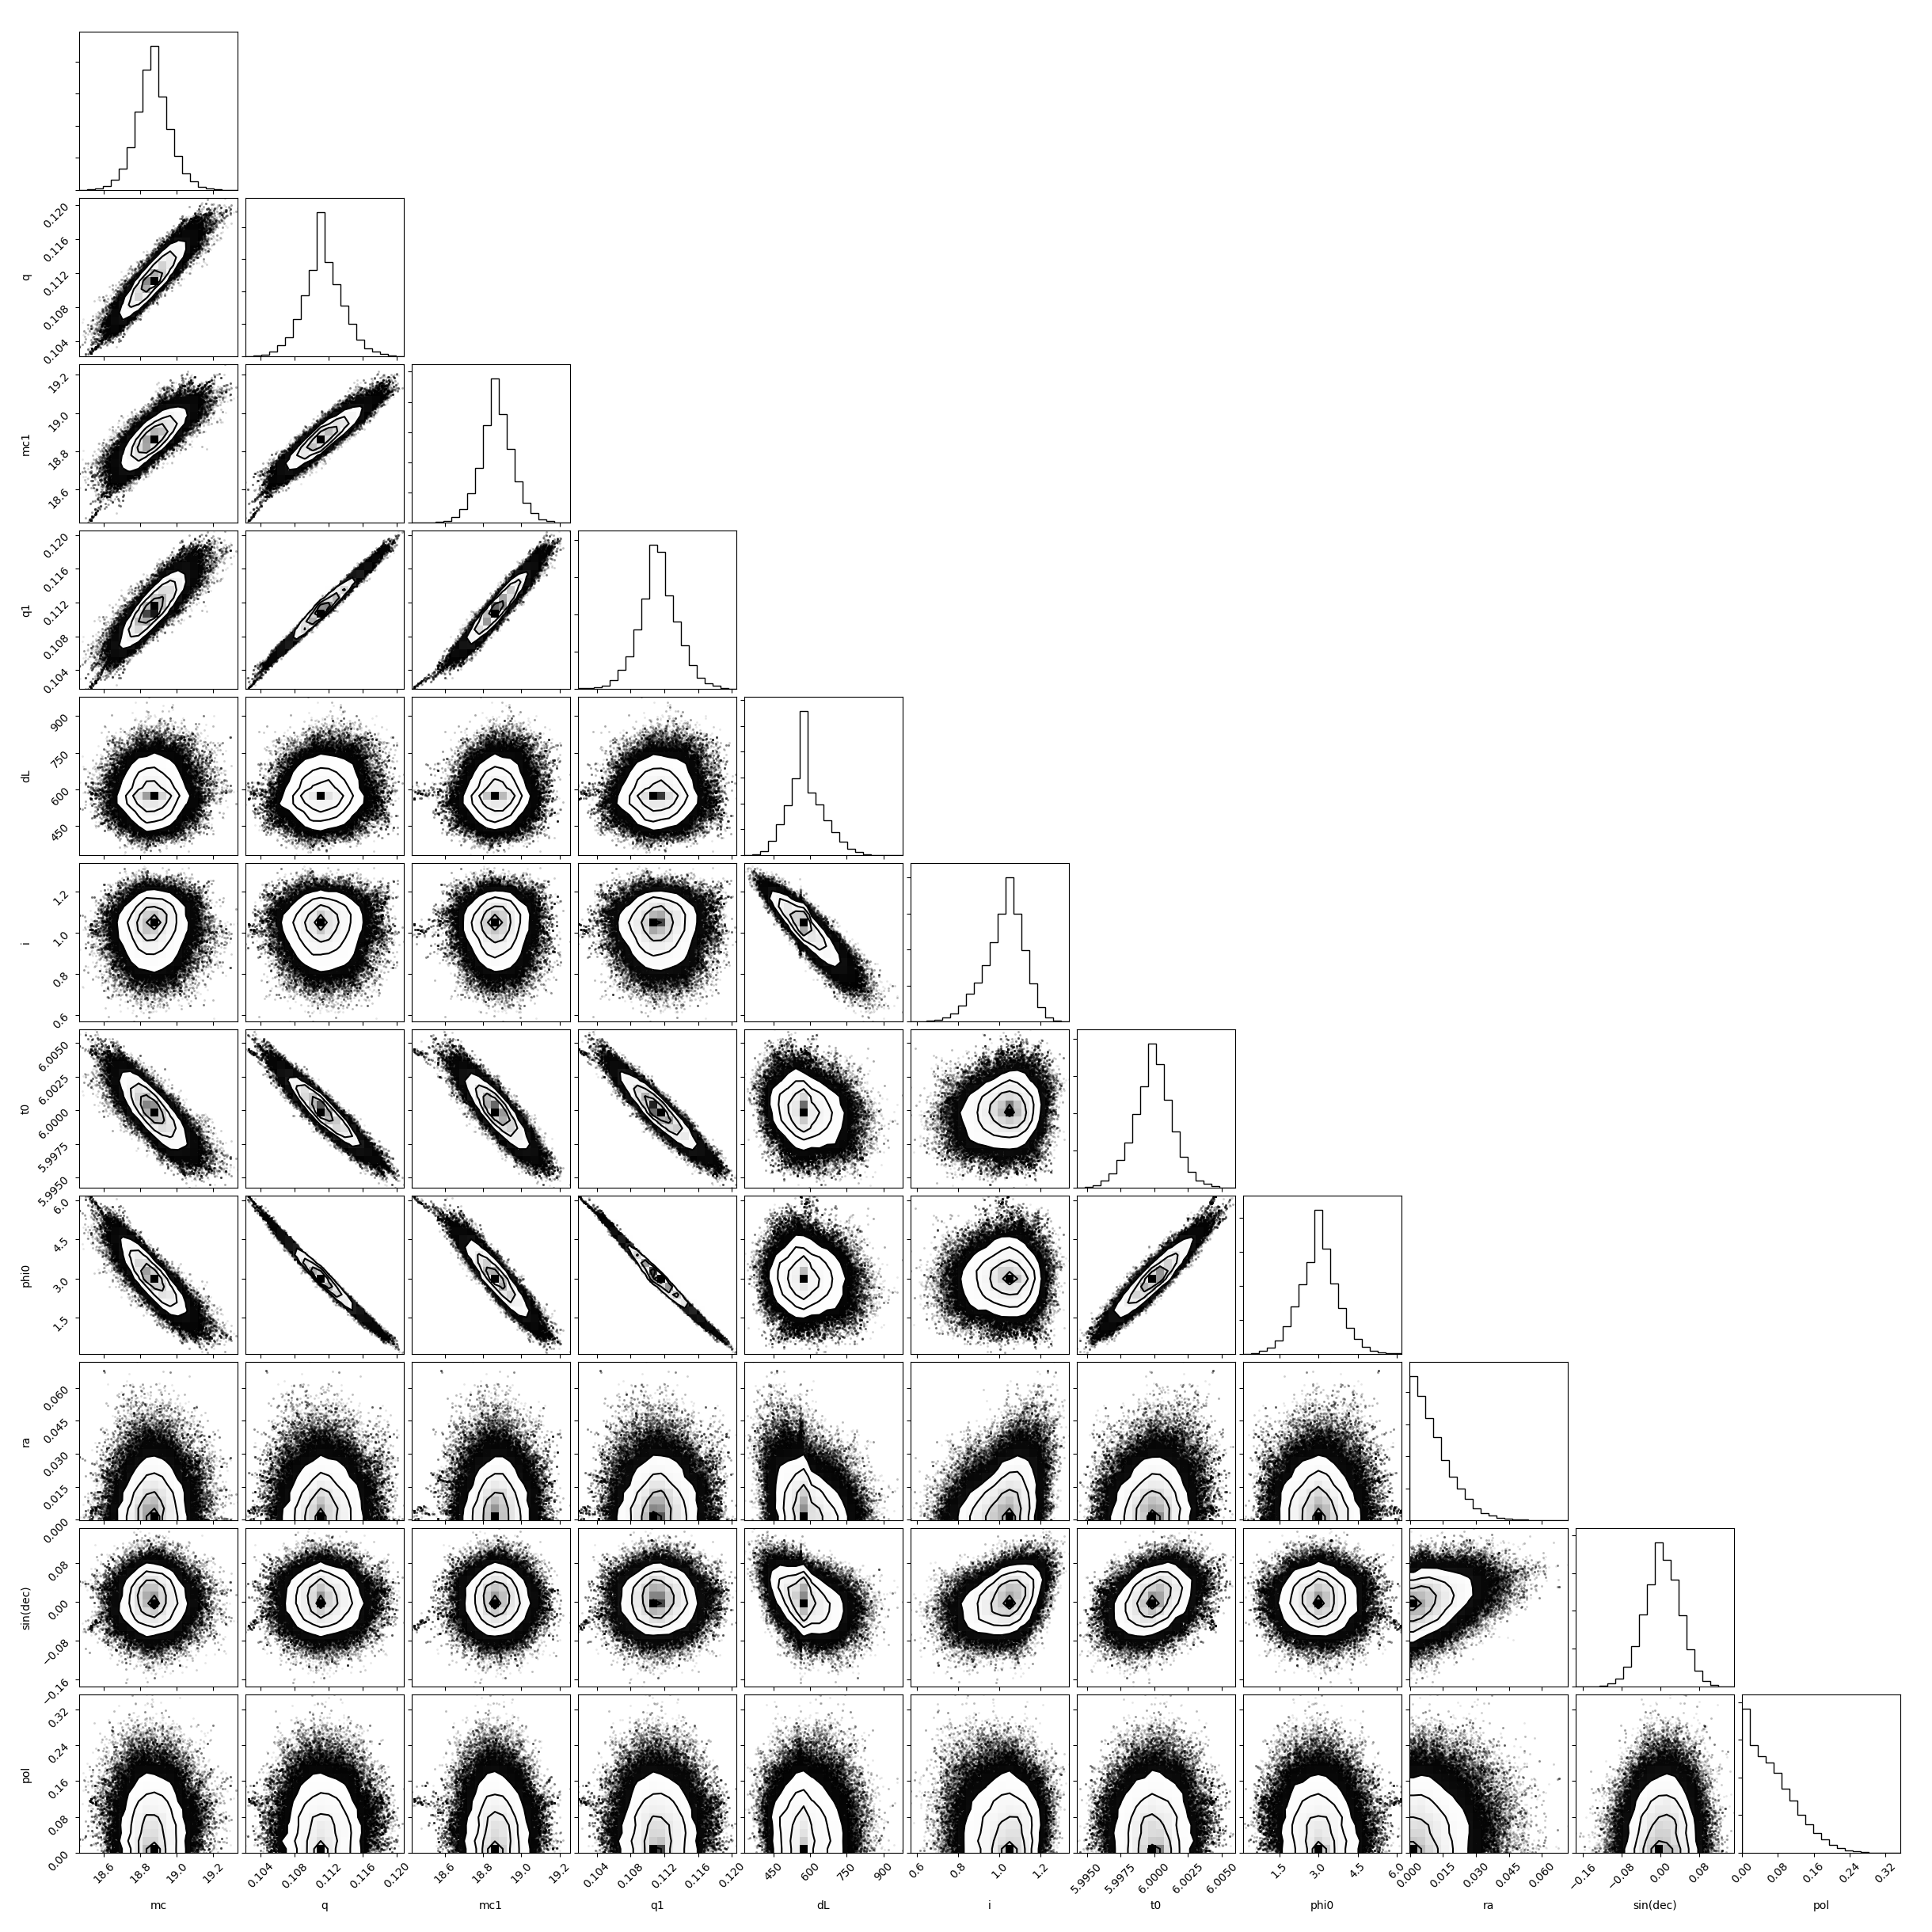
\includegraphics[scale=0.3]{figs/hp_hc_consistency_polarization_corner_plot_M_80_q_9_snr_25.png} 
    \end{center} 
    \caption{Corner plot for tests of GR based on checking for consistency between parameters ($M_{c}$, $q$, 
    $\Delta$ $M_{c}$ and $\Delta$ $q$) estimated from different polarizations. }
    \label{fig:hphc_corner}
\end{figure}

\newpage
.
\newpage

\begin{figure}[h]
    \begin{center}
    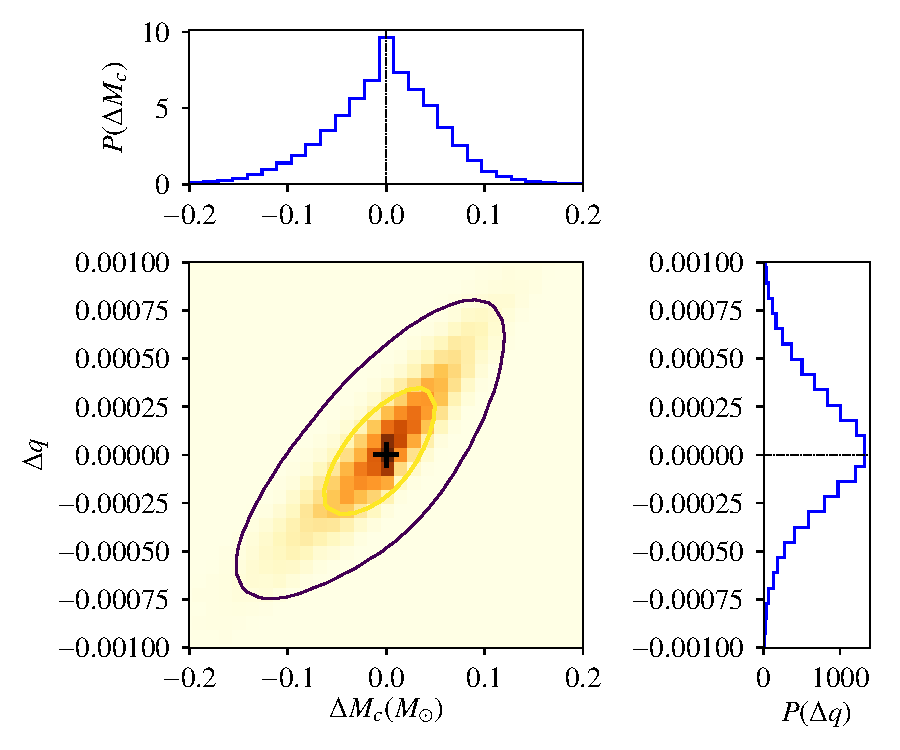
\includegraphics[scale=0.55]{figs/hp_hc_consistency_triangle_plot_delMc_delq_M_80_q_9_snr_25_pol.pdf} 
    \end{center} 
    \caption{The middle plot shows the 68\% and 95\% credible regions in joint posteriors of two parameters $\Delta$ $M_{c}$ and $\Delta$ $q$ estimated from different polarizations of simulated GR signal corresponding to a binary with total mass $M=80$ $M_{\odot}$ , mass ratio $q=9$ and SNR 25.}
    \label{fig:hphc_triangle}
\end{figure}

\begin{figure}[h]
    \begin{center}
    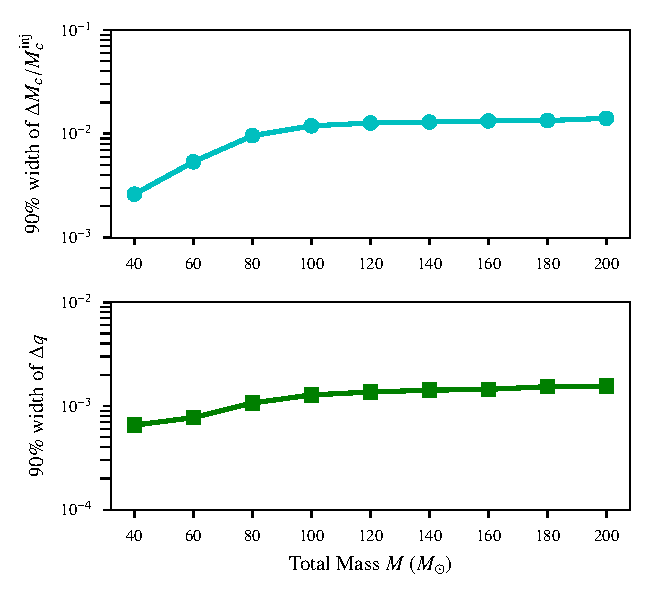
\includegraphics[scale=0.75]{figs/hp_hc_consistency_confidence_interval_varying_M.pdf} 
    \end{center} 
    \caption{The plots shows the width of the 90\% credible region of the $\Delta$ $M_{c}$ and $\Delta$ $q$ estimated from different polarizations of simulated GR signals for binaries with different total mass $M$. All binaries correspond to a mass ratio $q = 1/9$ and SNR 25.}
    \label{fig:hphc_bound_a}
\end{figure}

\newpage

\begin{figure}[]
    \begin{center}
    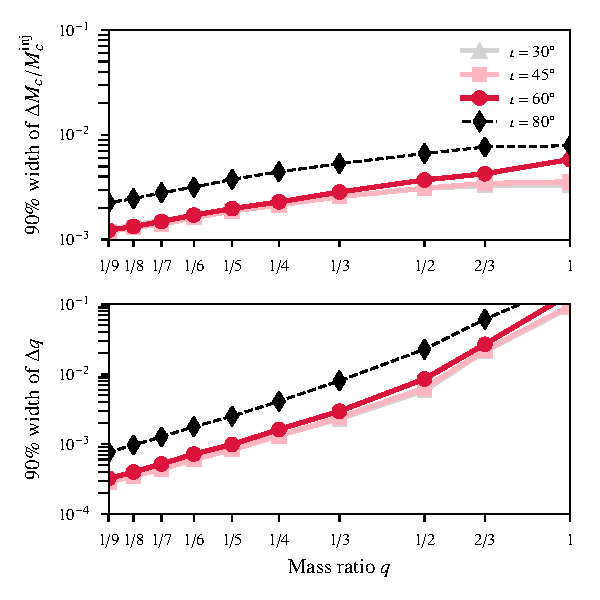
\includegraphics[scale=0.75]{figs/hp_hc_consistency_confidence_interval_varying_q.pdf} 
    \end{center} 
    \caption{The plots shows the width of the 90\% credible region of the $\Delta$ $M_{c}$ and $\Delta$ $q$ estimated from different polarizations of simulated GR signals for binaries with different total mass ratio $q$. All binaries correspond to a mass ratio $M=40$ $M_{\odot}$ and SNR 25.}
    \label{fig:hphc_bound_b}
\end{figure}


%%%%%%%%%%%%%%%%%%%%%%%%%%%%%%%%%%%%%%%%%%%%%%%%%%%%%%%%%%%%%%%%%%%%%%%%%%%%%%
\newpage

\subsection{Consistency between the amplitude of different polarizations}
\subsubsection{$v(f) = v$}
required (?)
\subsubsection{$v(f) = v f$}
In GR, the gravitational radiation could be written as a complex time series $\h(t)=h_+(t) - ih_\times(t)$. However, due to birefringence, one of the polarization can get amplified while the other one may get damped. We formulate a test for amplitude birefringence by introducing a coupling parameter $v$:
\begin{eqnarray} 
\h(f; \blambda) =  \Hat{h_+}(f; \blambda) - i \Hat{h_\times}(f; \blambda),
\label{eq:test_cs}
\end{eqnarray}
where $\Hat{h_+}(f; \blambda)=h^{GR}_+ + i v f h^{GR}_{\times}$ and $\Hat{h_\times}(f; \blambda)=h^{GR}_\times - i v f h^{GR}_{+}$.
Corner plot  - Fig \ref{fig:cs_corner};\\
triangle plot - Fig \ref{fig:cs_hist};\\
90\% credible intervals of $v$  - Fig \ref{fig:cs_bound};\\
modGR injection - Fig \ref{fig:cs_modgr};

\newpage

\begin{figure}[h!]
    \begin{center}
    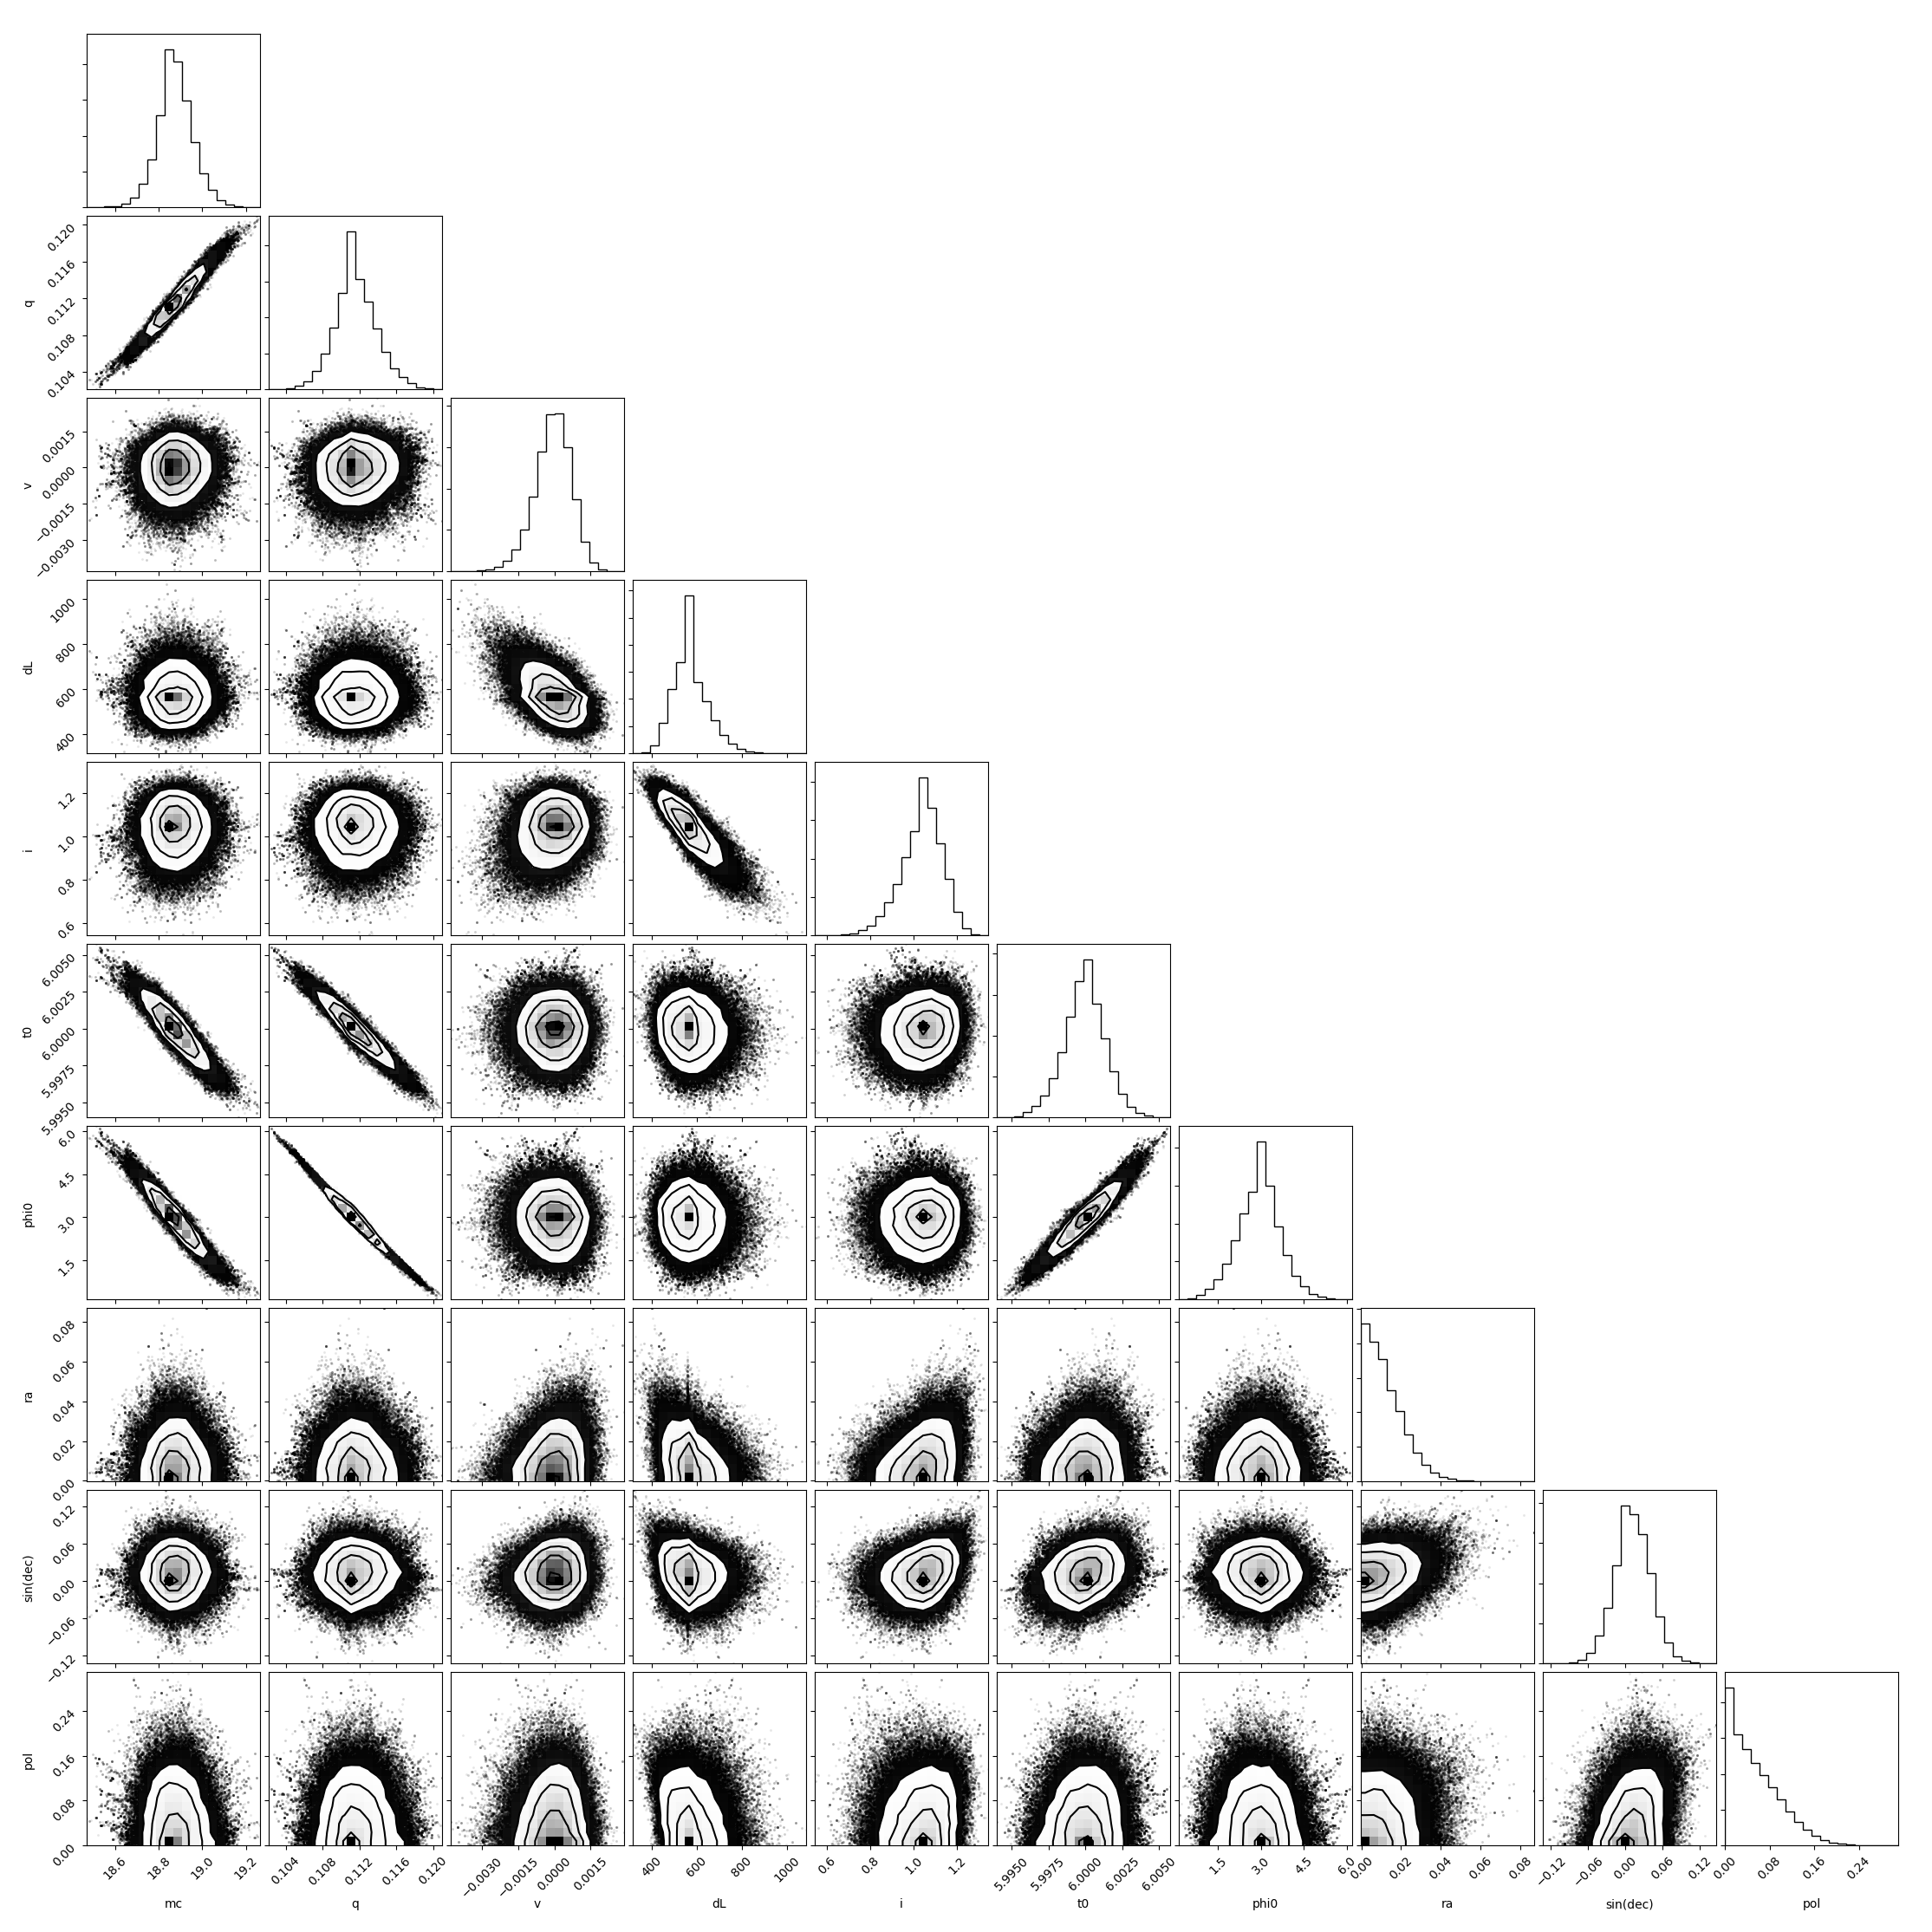
\includegraphics[scale=0.3]{figs/v1_80925_corner_plot.png} 
    \end{center} 
    \caption{Corner plot for tests of GR based on checking consistency between the amplitude of different polarization.}
    \label{fig:cs_corner}
\end{figure}

\newpage
.
\newpage

\begin{figure}[h!]
    \begin{center}
    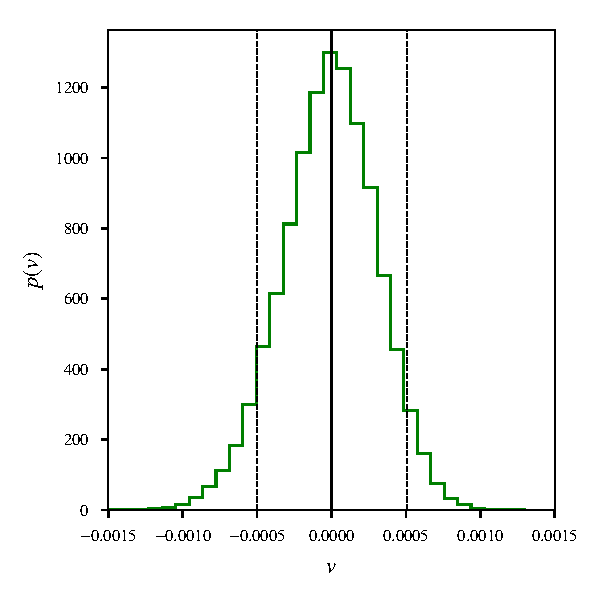
\includegraphics[scale=0.7]{figs/v1_GR_hist_M_80_q_9_dL_250.pdf} 
    \end{center} 
    \caption{Histogram of the deviation parameter $v$ estimated from simulated GR signal for binaries with $M=80$ $M_{\odot}$ and $q=1/9$. SNR fixed at 100.}
    \label{fig:cs_hist}
\end{figure}


\begin{figure}[h]
    \begin{center}
    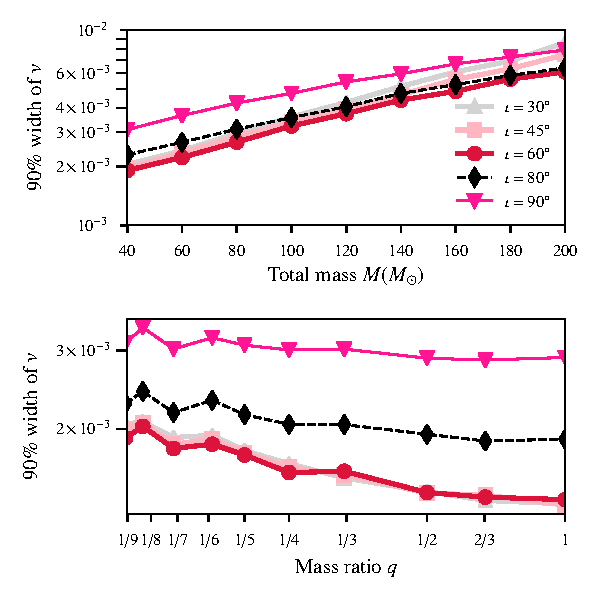
\includegraphics[scale=0.75]{figs/v1_confidence_interval_pol.pdf} 
    \end{center} 
    \caption{The plots shows the width of the 90\% credible region of the deviation parameter $v_1$ estimated from different polarizations of simulated GR signals for binaries with different total mass $M$ and mass ratio $q$. All binaries correspond to a SNR 25.}
    \label{fig:cs_bound}
\end{figure}

\newpage
\begin{figure}[h!]
    \begin{center}
    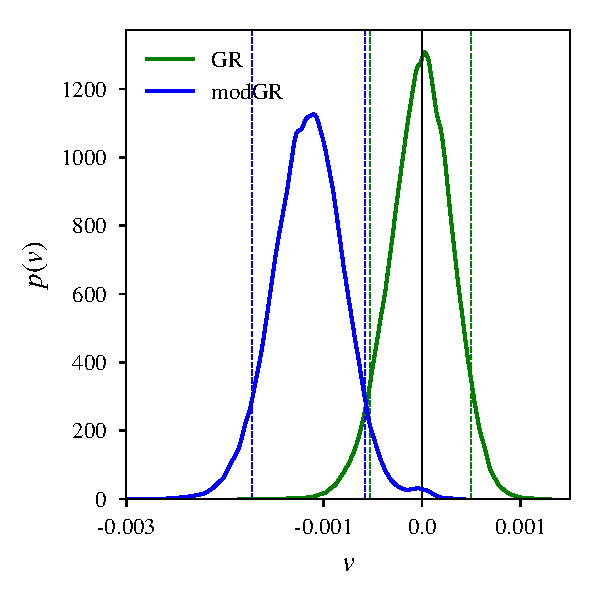
\includegraphics[scale=0.7]{figs/v1_modgr_hist_M_80_q_9_dL_250.pdf} \end{center} 
    \caption{Histograms of the deviation parameter $v$ estimated from simulated GR and modGR signal for binaries with $M=80$ $M_{\odot}$, $q=1/9$ and $dL=200$ Mpc.}
    \label{fig:cs_modgr}
\end{figure}

\bibliographystyle{apsrev-nourl}
\bibliography{TestGR}

\end{document}
